\documentclass[10pt,fleqn]{article}
\newcommand{\name}[1]{\def\psettitlename{#1}}
\newcommand{\course}[1]{\def\psettitlecourse{#1}}
\newcommand{\rsection}[1]{\def\psettitlersection{#1}}
\newcommand{\psetnum}[1]{\def\psettitlepsetnum{#1}}
%\usepackage[journal=rsc]{chemstyle}
%\usepackage{mhchem}
\usepackage{amsmath}
\usepackage{amssymb}
\usepackage{amsfonts}
\usepackage{esint}
\usepackage{bbm}
\usepackage{amscd}
\usepackage{picinpar}
\usepackage[pdftex]{graphicx}
\usepackage{tikz}
\usepackage{indentfirst}
\usepackage{wrapfig}
\usepackage{units}
\usepackage{textcomp}
\usepackage[utf8x]{inputenc}
% \usepackage{feyn}
\usepackage{feynmp}
\usetikzlibrary{
  arrows,
  calc,
  decorations.pathmorphing,
  decorations.pathreplacing,
  decorations.markings,
  fadings,
  positioning,
  shapes
}

\DeclareGraphicsRule{*}{mps}{*}{}
\newcommand{\ud}{\mathrm{d}}
\newcommand{\ue}{\mathrm{e}}
\newcommand{\ui}{\mathrm{i}}
\newcommand{\res}{\mathrm{Res}}
\newcommand{\Tr}{\mathrm{Tr}}
\newcommand{\dsum}{\displaystyle\sum}
\newcommand{\dprod}{\displaystyle\prod}
\newcommand{\dlim}{\displaystyle\lim}
\newcommand{\dint}{\displaystyle\int}
\newcommand{\fsno}[1]{{\!\not\!{#1}}}
\newcommand{\eqar}[1]
{
  \begin{align*}
    #1
  \end{align*}
}
\newcommand{\texp}[2]{\ensuremath{{#1}\times10^{#2}}}
\newcommand{\dexp}[2]{\ensuremath{{#1}\cdot10^{#2}}}
\newcommand{\eval}[2]{{\left.{#1}\right|_{#2}}}
\newcommand{\paren}[1]{{\left({#1}\right)}}
\newcommand{\lparen}[1]{{\left({#1}\right.}}
\newcommand{\rparen}[1]{{\left.{#1}\right)}}
\newcommand{\abs}[1]{{\left|{#1}\right|}}
\newcommand{\sqr}[1]{{\left[{#1}\right]}}
\newcommand{\crly}[1]{{\left\{{#1}\right\}}}
\newcommand{\angl}[1]{{\left\langle{#1}\right\rangle}}
\newcommand{\tpdiff}[4][{}]{{\paren{\frac{\partial^{#1} {#2}}{\partial {#3}{}^{#1}}}_{#4}}}
\newcommand{\tpsdiff}[4][{}]{{\paren{\frac{\partial^{#1}}{\partial {#3}{}^{#1}}{#2}}_{#4}}}
\newcommand{\pdiff}[3][{}]{{\frac{\partial^{#1} {#2}}{\partial {#3}{}^{#1}}}}
\newcommand{\diff}[3][{}]{{\frac{\ud^{#1} {#2}}{\ud {#3}{}^{#1}}}}
\newcommand{\psdiff}[3][{}]{{\frac{\partial^{#1}}{\partial {#3}{}^{#1}} {#2}}}
\newcommand{\sdiff}[3][{}]{{\frac{\ud^{#1}}{\ud {#3}{}^{#1}} {#2}}}
\newcommand{\tpddiff}[4][{}]{{\left(\dfrac{\partial^{#1} {#2}}{\partial {#3}{}^{#1}}\right)_{#4}}}
\newcommand{\tpsddiff}[4][{}]{{\paren{\dfrac{\partial^{#1}}{\partial {#3}{}^{#1}}{#2}}_{#4}}}
\newcommand{\pddiff}[3][{}]{{\dfrac{\partial^{#1} {#2}}{\partial {#3}{}^{#1}}}}
\newcommand{\ddiff}[3][{}]{{\dfrac{\ud^{#1} {#2}}{\ud {#3}{}^{#1}}}}
\newcommand{\psddiff}[3][{}]{{\frac{\partial^{#1}}{\partial{}^{#1} {#3}} {#2}}}
\newcommand{\sddiff}[3][{}]{{\frac{\ud^{#1}}{\ud {#3}{}^{#1}} {#2}}}
\usepackage{fancyhdr}
\usepackage{multirow}
\usepackage{fontenc}
%\usepackage{tipa}
\usepackage{ulem}
\usepackage{color}
\usepackage{cancel}
\newcommand{\hcancel}[2][black]{\setbox0=\hbox{#2}%
\rlap{\raisebox{.45\ht0}{\textcolor{#1}{\rule{\wd0}{1pt}}}}#2}
\pagestyle{fancy}
\setlength{\headheight}{67pt}
\fancyhead{}
\fancyfoot{}
\fancyfoot[C]{\thepage}
\fancyhead[R]
{
\psettitlename \\
\psettitlecourse{} Problem Set \psettitlepsetnum \\
\ifx\psettitlersection\empty
\else
Recitation Section \psettitlersection
\fi
}
\renewcommand{\footruleskip}{0pt}
\renewcommand{\headrulewidth}{0.4pt}
\renewcommand{\footrulewidth}{0pt}
\addtolength{\hoffset}{-1.3cm}
\addtolength{\voffset}{-2cm}
\addtolength{\textwidth}{3cm}
\addtolength{\textheight}{2.5cm}
\renewcommand{\footskip}{10pt}
\setlength{\headwidth}{\textwidth}
\setlength{\headsep}{20pt}
\setlength{\marginparwidth}{0pt}
\parindent=0pt
\psetnum{2}
\course{8.422}
\rsection{1}
\name{Yichao Yu}
\renewcommand{\thesection}{\arabic{section}.}
\renewcommand{\thesubsection}{(\alph{subsection})}
\renewcommand{\thesubsubsection}{\roman{subsubsection}.}

\begin{document}
\section{}
\subsection{}
\eqar{
  &\sqr{a^\dagger b-ab^\dagger, a^\dagger a+b^\dagger b}\\
  =&\sqr{a^\dagger b, a^\dagger a}-\sqr{ab^\dagger, a^\dagger a}+\sqr{a^\dagger b, b^\dagger b}-\sqr{ab^\dagger, b^\dagger b}\\
  =&a^\dagger\sqr{a^\dagger, a} b-\sqr{a, a^\dagger} ab^\dagger+a^\dagger \sqr{b, b^\dagger} b-ab^\dagger \sqr{b^\dagger, b}\\
  =&-a^\dagger b-ab^\dagger+a^\dagger b+ab^\dagger\\
  =&0
  \intertext{Therefore,}
  \sqr{B, n_a+n_b}=&\sqr{\exp\paren{\theta\paren{a^\dagger b-ab^\dagger}}, n_a+n_b}\\
  =&0\\
  B^\dagger=&\exp\paren{\theta\paren{a^\dagger b-ab^\dagger}^\dagger}\\
  =&\exp\paren{-\theta\paren{a^\dagger b-ab^\dagger}}\\
  =&B^{-1}
}
\subsection{}
\eqar{
  \exp\paren{\theta A}B\exp\paren{-\theta A}=&\sum_{nm}(-1)^m\frac{\theta^{n+m} A^nBA^m}{n!m!}\\
  =&\sum_{N}\sum^{N}_{m=0}(-1)^m\frac{\theta^N A^{N-m}BA^m}{(N-m)!m!}\\
  =&\sum_{N}\frac{\theta^N}{N!}\sum^{N}_{m=0}(-1)^m\frac{N! A^{N-m}BA^m}{(N-m)!m!}\\
  =&\sum_{N}\frac{\theta^N}{N!}\sqr{A, B}_N
  \intertext{where $\sqr{A, B}_N$ is defined as $\sqr{A, B}_N=\sqr{A, \sqr{A, B}_{N-1}}$ and $\sqr{A, B}_0=B$}
  \sqr{\paren{a^\dagger b-ab^\dagger}, a}_N=&\left\{
    \begin{array}{ll}
      (-1)^{N / 2}a&(2\mid N)\\
      (-1)^{(N + 1) / 2}b&(2\nmid N)
    \end{array}
  \right.\\
  \sqr{\paren{a^\dagger b-ab^\dagger}, b}_N=&\left\{
    \begin{array}{ll}
      (-1)^{N / 2}b&(2\mid N)\\
      (-1)^{(N - 1) / 2}a&(2\nmid N)
    \end{array}
  \right.\\
  BaB^{-1}=&\sum_{N}\frac{\theta^N}{N!}\sqr{\paren{a^\dagger b-ab^\dagger}, a}_N\\
  =&\sum_{n}\frac{\theta^{2n}}{(2n)!}\sqr{\paren{a^\dagger b-ab^\dagger}, a}_{2n}+
  \sum_{n}\frac{\theta^{2n+1}}{(2n+1)!}\sqr{\paren{a^\dagger b-ab^\dagger}, a}_{2n+1}\\
  =&\sum_{n}\frac{\theta^{2n}}{(2n)!}(-1)^na+\sum_{n}\frac{\theta^{2n+1}}{(2n+1)!}(-1)^{n+1}b\\
  =&\cos\theta a-\sin\theta b\\
  BbB^{-1}=&\sum_{N}\frac{\theta^N}{N!}\sqr{\paren{a^\dagger b-ab^\dagger}, b}_N\\
  =&\sum_{n}\frac{\theta^{2n}}{(2n)!}\sqr{\paren{a^\dagger b-ab^\dagger}, b}_{2n}+
  \sum_{n}\frac{\theta^{2n+1}}{(2n+1)!}\sqr{\paren{a^\dagger b-ab^\dagger}, b}_{2n+1}\\
  =&\sum_{n}\frac{\theta^{2n}}{(2n)!}(-1)^nb+\sum_{n}\frac{\theta^{2n+1}}{(2n+1)!}(-1)^{n}a\\
  =&\cos\theta b+\sin\theta a\\
  B|0, \alpha\rangle=&B\ue^{-\abs{\alpha}^2/2}\ue^{\alpha a^\dagger}|0, 0\rangle\\
  =&\ue^{-\abs{\alpha}^2/2}B\ue^{\alpha a^\dagger}B^{-1}B|0, 0\rangle\\
  =&\ue^{-\abs{\alpha}^2/2}\ue^{\alpha\paren{\cos\theta a^\dagger-\sin\theta b^\dagger}}|0, 0\rangle\\
  =&\ue^{-\abs{\alpha}^2/2}\ue^{\alpha\cos\theta a^\dagger}\ue^{-\alpha\sin\theta b^\dagger}|0, 0\rangle\\
  =&|-\alpha\sin\theta, \alpha\cos\theta\rangle
}
\subsection{}
\eqar{
  s_x=&a^\dagger b+ab^\dagger\\
  s_y=&-\ui\paren{a^\dagger b-ab^\dagger}\\
  B=&\ue^{\ui \theta s_y}
  \intertext{which is a rotation around $y$}
  &\paren{n_a+n_b}^2\\
  =&s_z^2+4a^\dagger ab^\dagger b\\
  =&s_z^2+4s^+s^-\\
  =&s_x^2+s_y^2+s_z^2\\
  =&S^2
  \intertext{which is the total spin}
  \sqr{s_x, s_y}=&\sqr{a^\dagger b+ab^\dagger, -\ui\paren{a^\dagger b-ab^\dagger}}\\
  =&-\ui\sqr{a^\dagger b+ab^\dagger, a^\dagger b-ab^\dagger}\\
  =&2\ui\sqr{a^\dagger b, ab^\dagger}\\
  =&2\ui a^\dagger a\sqr{b, b^\dagger}+2\ui\sqr{a^\dagger, a}b^\dagger b\\
  =&2\ui a^\dagger a-2\ui b^\dagger b\\
  =&2\ui s_z\\
  \sqr{s_y, s_z}=&\sqr{-\ui\paren{a^\dagger b-ab^\dagger}, a^\dagger a-b^\dagger b}\\
  =&-\ui a^\dagger \sqr{a^\dagger, a} b
  +\ui a^\dagger \sqr{b, b^\dagger} b
  +\ui\sqr{a, a^\dagger} ab^\dagger
  -\ui ab^\dagger \sqr{b^\dagger, b}\\
  =&2\ui s_x\\
  \sqr{s_z, s_x}=&\sqr{a^\dagger a-b^\dagger b, a^\dagger b+ab^\dagger}\\
  =&a^\dagger \sqr{a, a^\dagger} b
  +\sqr{a^\dagger, a} ab^\dagger
  -a^\dagger \sqr{b^\dagger, b} b
  -ab^\dagger \sqr{b, b^\dagger}\\
  =&2a^\dagger b - 2ab^\dagger\\
  =&2\ui s_y
}
\subsection{}
\eqar{
  B|0, n\rangle=&B\frac{{a^\dagger}^n}{n!}|0, 0\rangle\\
  =&\frac{\paren{a^\dagger-b^\dagger}^n}{2^{n/2}n!}|0, 0\rangle\\
  =&\sum_{i}\frac{{a^\dagger}^i{b^\dagger}^{n-i}}{2^{n/2}i!\paren{n-i}!}|0, 0\rangle\\
  =&\sum_{i}\frac{|n-i, i\rangle}{\sqrt{2^ni!\paren{n-i}!}}
  \intertext{The state(s) with the largest amplitude is $|n/2,n/2\rangle$ (when $n$ is even) or $|(n+1)/2,(n-1)/2\rangle$ and $|(n-1)/2,(n+1)/2\rangle$ when $n$ is odd}
}
The variance of the distribution is $\dfrac{n}{4}$ so the relative width is getting narrower for larger $n$ although the absolute width is getting wider.

\section{}
\subsection{}
\eqar{
  \paren{\Delta n'}^2=&\angl{{n'}^2}-\angl{n'}^2\\
  =&\abs{t}^4\paren{\Delta n}^2\\
  =&\abs{t}^4\abs{\alpha}^2\\
  \angl{n'}=&\abs{t}^2\abs{\alpha}^2\\
  >&\abs{t}^4\abs{\alpha}^2\qquad\text{(when $0<\abs{t}<1$ and $\alpha\neq0$)}
}
\subsection{}
As shown in problem one.
\eqar{
  \rho'=&\Tr_b\paren{B|0, \alpha\rangle\langle0, \alpha|B^\dagger}\\
  =&\Tr_b\paren{|r\alpha, t\alpha\rangle\langle r\alpha, t\alpha|}\\
  =&|t\alpha\rangle\langle t\alpha|
}

\section{}
\subsection{}
After the first beam splitter
\eqar{
  |\psi_1\rangle=&\frac{|0,1\rangle+|1,0\rangle}{\sqrt2}
  \intertext{After the phase shift}
  |\psi_2\rangle=&\frac{\ue^{-\ui\phi/2}|0,1\rangle+\ue^{\ui\phi/2}|1,0\rangle}{\sqrt2}
  \intertext{After the second beam splitter}
  |\psi_3\rangle=&\frac{\ue^{-\ui\phi/2}}{\sqrt2}\paren{\frac{|0,1\rangle-|1,0\rangle}{\sqrt2}}+\frac{\ue^{\ui\phi/2}}{\sqrt2}\paren{\frac{|0,1\rangle+|1,0\rangle}{\sqrt2}}\\
  =&\frac{\ue^{-\ui\phi/2}}{2}\paren{|0,1\rangle-|1,0\rangle}+\frac{\ue^{\ui\phi/2}}{2}\paren{|0,1\rangle+|1,0\rangle}\\
  =&\cos\frac{\phi}{2}|0,1\rangle+\ui\sin\frac{\phi}{2}|1,0\rangle\\
  P_b=&\cos^2\frac{\phi}{2}\\
  V=&\frac{\max\paren{P_b}-\min\paren{P_b}}{\max\paren{P_b}+\min\paren{P_b}}\\
  =&\frac{1-0}{1+0}\\
  =&1
}
\subsection{}
\eqar{
  |\psi_0\rangle=&|0, 1, 0\rangle\\
  |\psi_1\rangle=&\frac{|0, 0, 1\rangle+|0, 1, 0\rangle}{\sqrt2}\\
  |\psi_2\rangle=&\frac{1}{\sqrt2}\paren{\ue^{\ui\phi/2}|0, 0, 1\rangle+\ue^{-\ui\phi/2}\paren{\cos\theta|0, 1, 0\rangle+\sin\theta|1, 0, 0\rangle}}\\
  |\psi_3\rangle=&\frac{1}{\sqrt2}\paren{
    \ue^{\ui\phi/2}\frac{|0, 0, 1\rangle+|0, 1, 0\rangle}{\sqrt2}
    +\cos\theta\ue^{-\ui\phi/2}\frac{|0, 1, 0\rangle-|0, 0, 1\rangle}{\sqrt2}
    +\sin\theta\ue^{-\ui\phi/2}|1, 0, 0\rangle}\\
  =&\frac{\paren{\ue^{\ui\phi/2}-\cos\theta\ue^{-\ui\phi/2}}|0, 0, 1\rangle-\paren{\ue^{\ui\phi/2}+\cos\theta\ue^{-\ui\phi/2}}|0, 1, 0\rangle}{2}
  +\frac{\sin\theta\ue^{-\ui\phi/2}}{\sqrt2}|1, 0, 0\rangle\\
  P_b=&\abs{\frac{\ue^{\ui\phi/2}+\cos\theta\ue^{-\ui\phi/2}}{2}}^2\\
  =&\paren{\frac{1+\cos\theta}{2}\cos\frac{\phi}{2}}^2+\paren{\frac{1-\cos\theta}{2}\sin\frac{\phi}{2}}^2\\
  =&\frac{1+\cos^2\theta}{4}+\frac{\cos\theta}{2}\cos\phi\\
  V=&\frac{2\cos\theta}{1+\cos^2\theta}
}
\subsection{}
\eqar{
  |\psi_0\rangle=&|0, 0, 1, 0\rangle\\
  |\psi_1\rangle=&\frac{|0, 1, 0, 0\rangle+|0, 0, 1, 0\rangle}{\sqrt2}\\
  |\psi_2\rangle=&\frac{1}{\sqrt2}\paren{\ue^{\ui\phi/2}|0, 1, 0, 0\rangle+\ue^{-\ui\phi/2}|0, 0, 1, 0\rangle}\\
  |\psi_3\rangle=&\frac{\ue^{\ui\phi/2}}{\sqrt2}\paren{\cos\theta|0, 1, 0, 0\rangle+\sin\theta|1, 0, 0, 0\rangle}+\frac{\ue^{-\ui\phi/2}}{\sqrt2}\paren{\cos\theta'|0, 0, 1, 0\rangle+\sin\theta'|0, 0, 0, 1\rangle}\\
  =&\frac{\ue^{\ui\phi/2}\sin\theta}{\sqrt2}|1, 0, 0, 0\rangle
  +\frac{\ue^{-\ui\phi/2}\sin\theta'}{\sqrt2}|0, 0, 0, 1\rangle
  +\frac{\ue^{\ui\phi/2}\cos\theta}{\sqrt2}|0, 1, 0, 0\rangle
  +\frac{\ue^{-\ui\phi/2}\cos\theta'}{\sqrt2}|0, 0, 1, 0\rangle\\
  |\psi_4\rangle=&\frac{\ue^{\ui\phi/2}\sin\theta}{\sqrt2}|1, 0, 0, 0\rangle
  +\frac{\ue^{-\ui\phi/2}\sin\theta'}{\sqrt2}|0, 0, 0, 1\rangle\\
  &+\frac{\ue^{\ui\phi/2}\cos\theta}{2}\paren{|0, 0, 1, 0\rangle+|0, 1, 0, 0\rangle}
  +\frac{\ue^{-\ui\phi/2}\cos\theta'}{2}\paren{|0, 0, 1, 0\rangle-|0, 1, 0, 0\rangle}\\
  =&\frac{\ue^{\ui\phi/2}\sin\theta}{\sqrt2}|1, 0, 0, 0\rangle
  +\frac{\ue^{-\ui\phi/2}\sin\theta'}{\sqrt2}|0, 0, 0, 1\rangle\\
  &+\frac{\ue^{\ui\phi/2}\cos\theta+\ue^{-\ui\phi/2}\cos\theta'}{2}|0, 0, 1, 0\rangle
  +\frac{\ue^{\ui\phi/2}\cos\theta-\ue^{-\ui\phi/2}\cos\theta'}{2}|0, 1, 0, 0\rangle
  \intertext{Maximum and minimum probabilities}
  \max{P_b}=&\frac14\paren{\cos\theta+\cos\theta'}^2\\
  \min{P_b}=&\frac14\paren{\cos\theta-\cos\theta'}^2\\
  V=&\frac{2\cos\theta\cos\theta'}{\cos^2\theta+\cos^2\theta'}
}
Changing to condition probability does not change the visibility.

\subsection{}
\eqar{
  |\psi_0\rangle=&|0, 0, \alpha, 0\rangle\\
  |\psi_1\rangle=&|0, \frac\alpha2, \frac\alpha2, 0\rangle\\
  |\psi_2\rangle=&|0, \ue^{\ui\phi/2}\frac\alpha2, \ue^{-\ui\phi/2}\frac\alpha2, 0\rangle\\
  |\psi_3\rangle=&|\ue^{\ui\phi/2}\sin\theta\frac\alpha2, \ue^{\ui\phi/2}\cos\theta\frac\alpha2, \ue^{-\ui\phi/2}\cos\theta'\frac\alpha2, \ue^{-\ui\phi/2}\sin\theta'\frac\alpha2\rangle\\
  |\psi_4\rangle=&|\ue^{\ui\phi/2}\sin\theta\frac\alpha2, \ue^{\ui\phi/2}\cos\theta\frac\alpha2-\ue^{-\ui\phi/2}\cos\theta'\frac\alpha2, \ue^{\ui\phi/2}\cos\theta\frac\alpha2+\ue^{-\ui\phi/2}\cos\theta'\frac\alpha2, \ue^{-\ui\phi/2}\sin\theta'\frac\alpha2\rangle
  \intertext{Maximum and minimum intensity}
  \max{P_b}=&\frac{\alpha^2}4\paren{\cos\theta+\cos\theta'}^2\\
  \min{P_b}=&\frac{\alpha^2}4\paren{\cos\theta-\cos\theta'}^2\\
  V=&\frac{2\cos\theta\cos\theta'}{\cos^2\theta+\cos^2\theta'}
}

\section{}
\subsection{}
From the definition of entangled state, the state is a product state if Schmidt number is $1$. If a product state has a Schmidt number greater than $1$
\eqar{
  |\psi_A\rangle|\psi_B\rangle=&\sum_k\lambda_k|k_A\rangle|k_B\rangle\\
  |\psi_A\rangle=&\sum_k\lambda_k\langle\psi_B|k_B\rangle|k_A\rangle\\
  |\psi_B\rangle=&\sum_k\lambda_k\langle\psi_A|k_A\rangle|k_B\rangle\\
  |\psi_A\rangle|\psi_B\rangle=&\sum_{k_1,k_2}\lambda_{k_1}\langle\psi_B|{k_1}_B\rangle|{k_1}_A\rangle\lambda_{k_2}\langle\psi_A|{k_2}_A\rangle|{k_2}_B\rangle\\
  \neq&\sum_k\lambda_k|k_A\rangle|k_B\rangle
}
\subsection{}
With the same local unitary transformation on the right hand side, it is still a valid expansion of the new state and therefore the Schmidt number does not change.
\subsection{}
\eqar{
  \begin{array}{|c|c|}
    \hline
    \text{State}&\text{Schmidt number}\\\hline
    \phi_1&3\\\hline
    \phi_2&1\\\hline
    \phi_3&2\\\hline
    \phi_4&2\\\hline
  \end{array}
}
\subsection{}
Schmidt number is $2$.
\eqar{
  |\phi_1\rangle=&B|\psi\rangle\\
  =&\frac{1}{\sqrt{n!(n-1)!}2^n}\paren{\paren{a^\dagger+b^\dagger}^{n}\paren{a^\dagger-b^\dagger}^{n-1}+\paren{a^\dagger+b^\dagger}^{n-1}\paren{a^\dagger-b^\dagger}^{n}}|0,0\rangle\\
  =&\frac{1}{\sqrt{n!(n-1)!}2^{n-1}}\paren{a^\dagger+b^\dagger}^{n-1}a^\dagger\paren{a^\dagger-b^\dagger}^{n-1}|0,0\rangle\\
  =&\frac{1}{\sqrt{n!(n-1)!}2^{n-1}}\paren{{a^\dagger}^2-{b^\dagger}^2}^{n-1}a^\dagger|0,0\rangle
}
Therefore the Schmidt number is $n$. This is a better measure since these are the states that interfere later.

The Schmidt number for a coherent state after a beam splitter is $1$ since it is still a product state.

\subsection{}
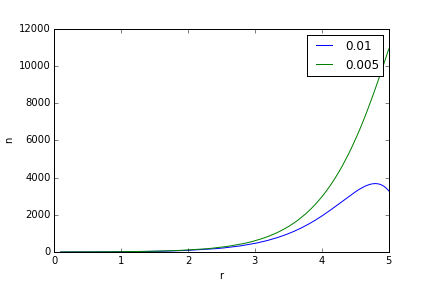
\includegraphics[width=12cm]{4.png}

\end{document}
